% Converted from the supplied Word draft and completed from saved experiment results.
\documentclass[letterpaper]{article}
\usepackage[T1]{fontenc}
\usepackage{aaai24}
\usepackage{times}
\usepackage{helvet}
\usepackage{courier}
\usepackage[hyphens]{url}
\usepackage{graphicx}
\urlstyle{rm}
\def\UrlFont{\rm}
\usepackage{natbib}
\usepackage{caption}
\usepackage{amsmath}
\usepackage{amssymb}
\usepackage{booktabs}
\usepackage{listings}
\lstset{
    basicstyle=\footnotesize\ttfamily,
    keywordstyle=\ttfamily,
    commentstyle=\ttfamily,
    stringstyle=\ttfamily,
    showstringspaces=false,
    keepspaces=true,
    columns=fullflexible,
    tabsize=4,
    breaklines=true,
    frame=tb,
    captionpos=t
}
\captionsetup[lstlisting]{justification=raggedright,singlelinecheck=false}
\frenchspacing
\setlength{\pdfpagewidth}{8.5in}
\setlength{\pdfpageheight}{11in}
\ifdefined\pdfinfo
\pdfinfo{/TemplateVersion (2024.1)}
\fi
\setcounter{secnumdepth}{1}
% Course assignment, rather than an AAAI proceedings publication.
\nocopyright
\title{AI6103 Assignment: Hyperparameter Analysis of EfficientNetV2-S}
\author{Zhang Mufan}
\affiliations{
    Nanyang Technological University\\
    mufan001@e.ntu.edu.sg\\
    G2505269G
}
\begin{document}
\maketitle
% Keep heading and paragraph spacing natural instead of stretching each column.
\raggedbottom
\begin{abstract}
In this project, eight experiments in total evaluate the effects of learning rate, cosine annealing, weight decay, and Mixup on dog breed classification with EfficientNetV2-S trained from scratch. A learning rate of 0.05 achieves the lowest training cross-entropy among the three rates tested over 15 epochs. Extending training to 300 epochs with cosine annealing further reduces training loss, while validation accuracy remains below 20\%. Adding weight decay of \(5 \times 10^{- 4}\) increases the best validation accuracy from 19.90\% to 34.77\%. Mixup with \(\alpha = 0.2\) further improves this figure to 38.62\%, and the selected checkpoint achieves 37.55\% test accuracy. The training curves show that weight decay and Mixup improve validation performance despite higher training losses.
\end{abstract}

\section{Introduction}

Some dog breeds look quite similar. The classifier therefore needs to pick up small visual differences that remain useful on new images. For a network trained from scratch, the learning rate and its schedule shape the optimization trajectory, while regularization influences the solutions reached during training. These effects can be distinguished through training and validation curves: decreasing training loss accompanied by increasing validation loss indicates that improved training-set fitting is no longer producing better predictions on held-out data. EfficientNetV2-S~\citep{tan2021efficientnetv2} provides the architecture for examining this relationship on the 120-class Dog Breed Identification dataset.

Eight experiments compare three initial learning rates, constant and cosine learning rate schedules, two weight decay coefficients, and Mixup augmentation. The learning rate study establishes the starting configuration for longer training, followed by comparisons of scheduling and regularization. Weight decay penalizes parameter magnitude, while Mixup trains the classifier on interpolated images and labels, encouraging smoother predictions between training examples. Training and validation cross-entropy and accuracy are tracked throughout these experiments to examine convergence, the emergence of overfitting, and the effects of regularization on predictive performance.

\begin{figure*}[t]
\centering
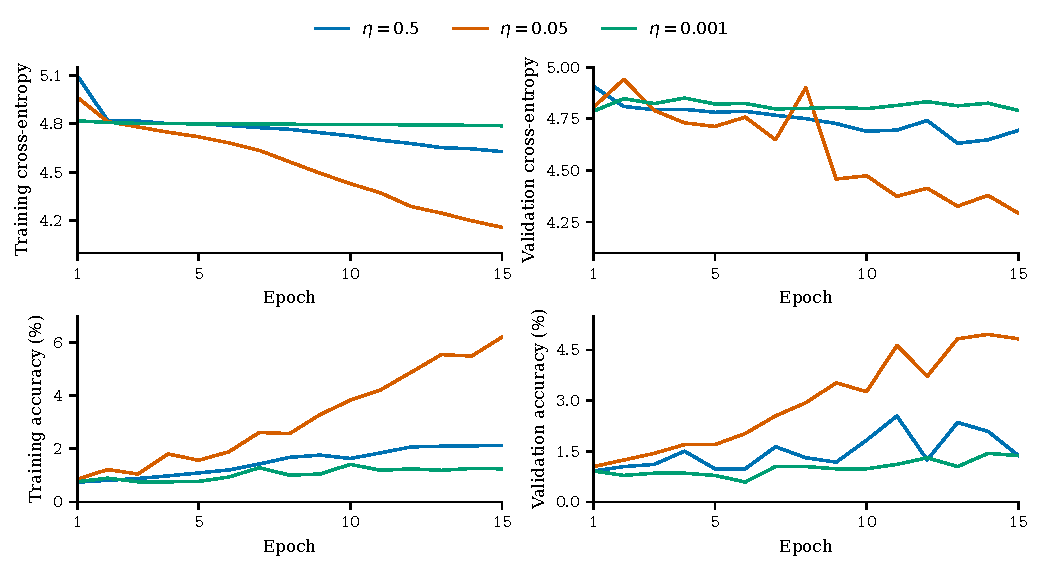
\includegraphics[width=\textwidth]{images/learning_rates.pdf}
\caption{Training and validation cross-entropy and accuracy for the three learning rates over 15 epochs. Accuracy is expressed as a percentage.}
\label{fig:learning-rates}
\end{figure*}

\section{Experimental Setup and Data Preprocessing}
\label{sec:setup}

All experiments in this assignment use the torchvision implementation of EfficientNetV2-S with randomly initialized weights. The final classification layer is replaced with a 120-class linear layer. Training uses SGD with momentum 0.9 and a batch size of 128. BF16 mixed precision is used during training, while validation and testing use FP32. The random seed is set to 6103, with deterministic algorithms enabled.

The dataset contains 10,222 images, divided into 7,155 training images, 1,533 validation images, and 1,534 test images according to the supplied split. Each image is converted to RGB and resized to \(100 \times 100\) using bilinear interpolation. Channel statistics are computed over the resized training images, with pixel values scaled to $[0,1]$. The resulting means and population standard deviations are shown in Table~\ref{tab:statistics}. Normalization is applied independently to each channel:

\begin{equation}
\widehat{x}_{c,h,w}=\frac{x_{c,h,w}-\mu_c}{\sigma_c}.
\label{eq:normalization}
\end{equation}

\begin{table}[ht]
\centering
\caption{Channel statistics computed from the training set.}
\label{tab:statistics}
\begin{tabular}{@{}lrr@{}}
\toprule
Channel & Mean $\mu_c$ & Standard deviation $\sigma_c$ \\
\midrule
Red & 0.477183 & 0.253416 \\
Green & 0.452764 & 0.247967 \\
Blue & 0.392786 & 0.252267 \\
\bottomrule
\end{tabular}
\end{table}

Training augmentation applies 12-pixel zero padding on each side, followed by a random \(100 \times 100\) crop and horizontal flipping with probability 0.5. The augmented images are converted to tensors and normalized using the training-set channel statistics. Validation and test images undergo resizing, tensor conversion, and normalization.

Listing~\ref{lst:preprocessing} shows the preprocessing code. Here, \texttt{stats} contains the training-set statistics in Table~\ref{tab:statistics}, and \texttt{training} is false for validation and test images.

\begin{lstlisting}[language=Python,float=!t,label={lst:preprocessing},caption={Preprocessing transforms used in the experiments. Images are converted to RGB before applying the transforms.}]
from torchvision import transforms as T

def make_transform(cfg, stats, training):
    size = cfg["image_size"]
    mode = T.InterpolationMode.BILINEAR
    ops = [T.Resize((size, size),
                    interpolation=mode,
                    antialias=True)]
    if training:
        ops += [
            T.Pad(cfg["padding"], fill=0,
                  padding_mode="constant"),
            T.RandomCrop(size),
            T.RandomHorizontalFlip(
                cfg["flip_probability"])]
    return T.Compose(ops + [
        T.ToTensor(),
        T.Normalize(
            stats["mean"], stats["std"])])
\end{lstlisting}

A content audit identifies 10 groups of byte-identical images spanning different splits and six duplicate-content groups with conflicting labels. The supplied split membership and labels are retained throughout the experiments.

Training metrics are accumulated online over augmented minibatches, while validation metrics are computed on unaugmented images in evaluation mode. Reported losses are cross-entropy values without the weight decay penalty. For Mixup, training loss and accuracy are weighted by the mixing coefficient against both paired labels. The initial learning rate is selected by final training cross-entropy; subsequent configurations and checkpoints are selected by validation accuracy, with lower validation cross-entropy and earlier epochs breaking ties.

\begin{figure*}[t]
\centering
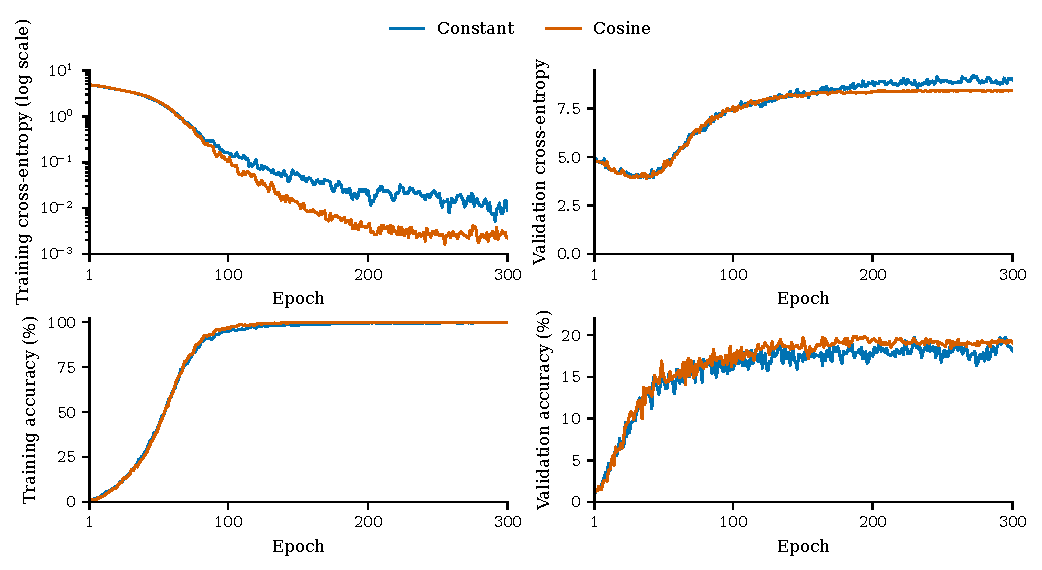
\includegraphics[width=\textwidth]{images/schedules.pdf}
\caption{Constant and cosine schedules over 300 epochs without weight decay. Training cross-entropy uses a logarithmic vertical axis to show late-stage differences.}
\label{fig:schedules}
\end{figure*}

\section{Initial Learning Rate}

In this assignment, three constant learning rates, 0.5, 0.05, and 0.001, are compared over 15 epochs without weight decay or learning rate scheduling. The remaining settings follow Section~\ref{sec:setup}. Table~\ref{tab:learning-rates} reports the metrics recorded at the end of epoch 15.

\begin{table}[ht]
\centering
\caption{Training and validation performance after 15 epochs.}
\label{tab:learning-rates}
\begin{tabular}{@{}lrrrr@{}}
\toprule
LR & Train CE & Val CE & \shortstack{Train acc.\\(\%)} & \shortstack{Val acc.\\(\%)} \\
\midrule
0.5 & 4.6273 & 4.6938 & 2.12 & 1.37 \\
0.05 & 4.1588 & 4.2930 & 6.21 & 4.83 \\
0.001 & 4.7874 & 4.7906 & 1.24 & 1.37 \\
\bottomrule
\end{tabular}
\end{table}

A learning rate of 0.05 performs best on all four final metrics. Figure~\ref{fig:learning-rates} shows a sustained decrease in its training loss and an overall increase in training and validation accuracy. The 0.5 run also reduces training loss, but progresses more slowly after the initial epochs and produces fluctuating validation accuracy. With 0.001, both loss curves remain nearly flat.

The final training cross-entropy at 0.001, 4.7874, is close to the uniform-prediction loss, \(\ln(120) \approx 4.7875\). This run makes little progress in 15 epochs. The updates appear too small to learn quickly from random initialization. With 0.5, the updates may be too large and slow down early optimization. For this task, 0.05 gives the lowest final training cross-entropy among the three tested rates and is used in the following experiments.

\begin{figure*}[t]
\centering
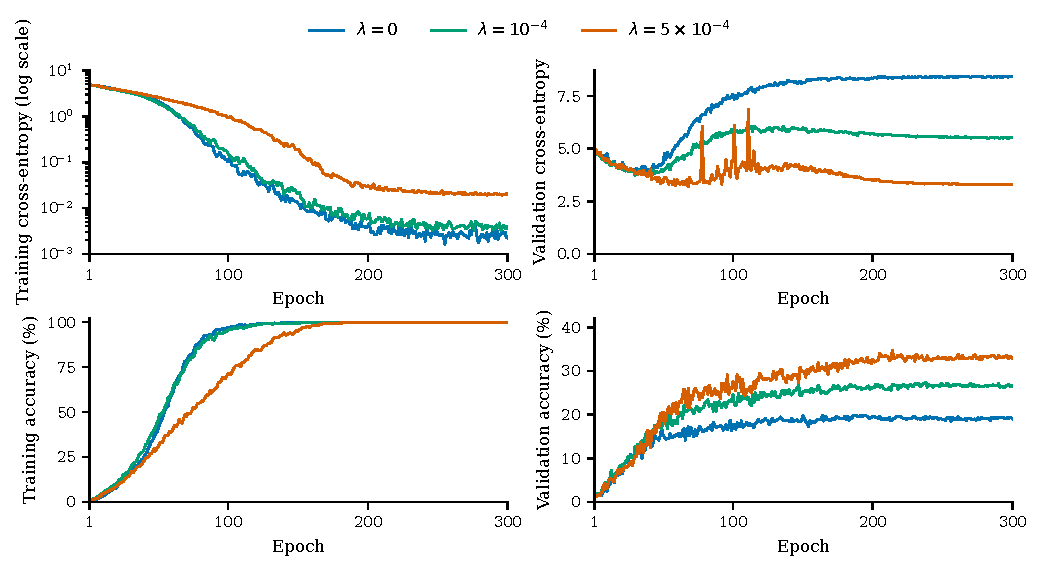
\includegraphics[width=\textwidth]{images/weight_decay.pdf}
\caption{Weight decay comparison under cosine annealing. Each curve contains the 300 recorded epoch metrics; training cross-entropy uses a logarithmic vertical axis.}
\label{fig:weight-decay}
\end{figure*}

\section{Learning Rate Schedule}

Cosine annealing gradually reduces the learning rate along a half-cosine curve, allowing larger updates early in training and smaller updates during later refinement~\citep{loshchilov2017sgdr}. The schedule is defined as

\begin{equation}
\eta_t=\frac{\eta_0}{2}\left[1+\cos\left(\frac{\pi t}{T}\right)\right],
\label{eq:cosine}
\end{equation}
where \(\eta_0=0.05\), \(T=300\), and \(t\) denotes the number of completed epochs. The learning rate is updated after each epoch and reaches zero at the end of training. A single cosine cycle is applied without restarts.

Two experiments compare this schedule with a constant learning rate of \(0.05\). Both run for 300 epochs without weight decay, with the remaining settings unchanged. Table~\ref{tab:schedules} reports the final metrics.

\begin{table}[ht]
\centering
\caption{Performance after 300 epochs under constant and cosine learning rate schedules.}
\label{tab:schedules}
\begin{tabular}{@{}lrrrr@{}}
\toprule
Schedule & Train CE & Val CE & \shortstack{Train acc.\\(\%)} & \shortstack{Val acc.\\(\%)} \\
\midrule
Constant & 0.0088 & 8.9741 & 99.66 & 18.13 \\
Cosine & 0.0022 & 8.4297 & 99.97 & 19.05 \\
\bottomrule
\end{tabular}
\end{table}


Figure~\ref{fig:schedules} shows that both schedules fit the training set closely, reaching more than 99.6\% training accuracy. Cosine annealing reduces final training cross-entropy from 0.0088 to 0.0022, or by 74.5\%. The validation gain is small: 0.91 percentage points. The best validation accuracies are also similar: 19.70\% for the constant schedule and 19.90\% for cosine annealing.

Validation cross-entropy reaches its minimum at epoch 40 under the constant schedule and epoch 38 under cosine annealing, then increases while training loss continues to decrease. The final validation losses, 8.9741 and 8.4297, indicate that prolonged optimization increasingly favors training-set fitting. Cross-entropy depends on the probability assigned to the true class, whereas top-1 accuracy depends only on the highest-scoring class. Consequently, validation loss can increase substantially without a comparable change in accuracy. The smaller late-stage updates improve optimization, but do little to resolve the generalization gap in the unregularized model.

\section{Weight Decay}

Weight decay discourages large parameter magnitudes. In the SGD implementation used here, the coefficient $\lambda$ adds an $L_2$ penalty to the minibatch objective:
\begin{equation}
\mathcal{L}_{\lambda}(w)=\mathcal{L}_{\mathrm{CE}}(w)
 +\frac{\lambda}{2}\lVert w\rVert_2^2.
\label{eq:weight-decay}
\end{equation}
With momentum 0.9, the parameter update is
\begin{equation}
\begin{aligned}
v_{k+1}&=0.9v_k+\nabla_w\mathcal{L}_{\mathrm{CE},k}(w_k)+\lambda w_k,\\
w_{k+1}&=w_k-\eta_k v_{k+1},
\end{aligned}
\label{eq:momentum}
\end{equation}
where $v_0=0$, $k$ indexes minibatches, and $\eta_k$ follows the epoch-level cosine schedule. Thus, parameter shrinkage contributes to the momentum buffer alongside the data gradient.

Two runs use $\lambda=5\times10^{-4}$ and $\lambda=10^{-4}$, respectively, with an initial learning rate of 0.05 and 300 training epochs. Table~\ref{tab:weight-decay} compares their final metrics with the cosine run without weight decay.

Both coefficients improve validation performance despite higher training cross-entropy. The stronger coefficient reduces final validation cross-entropy from 8.4297 to 3.2910 and raises final validation accuracy by 13.83 percentage points. The weaker coefficient produces an intermediate result, reaching 26.61\% validation accuracy.

Figure~\ref{fig:weight-decay} shows that stronger weight decay slows the initial reduction in training loss and delays the rise in training accuracy. Validation accuracy subsequently exceeds that of both alternatives, while validation cross-entropy remains much lower. By the final epoch, all three runs classify almost every augmented training example correctly, yet their validation performance differs substantially. The advantage therefore lies in the learned predictive behavior beyond the training images, rather than a lower final training error. The $L_2$ penalty counteracts the tendency to fit the training data through increasingly large parameters and reduces the severe validation-loss growth seen without weight decay.

\begin{table}[ht]
\centering
\caption{Final metrics after 300 epochs with cosine annealing and different weight decay coefficients. Accuracy is in percent.}
\label{tab:weight-decay}
\begin{tabular}{@{}lrrrr@{}}
\toprule
$\lambda$ & Train CE & Val CE & \shortstack{Train acc.\\(\%)} & \shortstack{Val acc.\\(\%)} \\
\midrule
0 & 0.0022 & 8.4297 & 99.97 & 19.05 \\
$10^{-4}$ & 0.0036 & 5.5271 & 99.96 & 26.61 \\
$5\times10^{-4}$ & 0.0199 & 3.2910 & 99.99 & 32.88 \\
\bottomrule
\end{tabular}
\end{table}

The best validation accuracies are 19.90\%, 27.33\%, and 34.77\% for $\lambda=0$, $10^{-4}$, and $5\times10^{-4}$, respectively. The strongest coefficient reaches its best validation accuracy at epoch 214 and is selected as the baseline for the Mixup experiment.

\begin{figure*}[t]
\centering
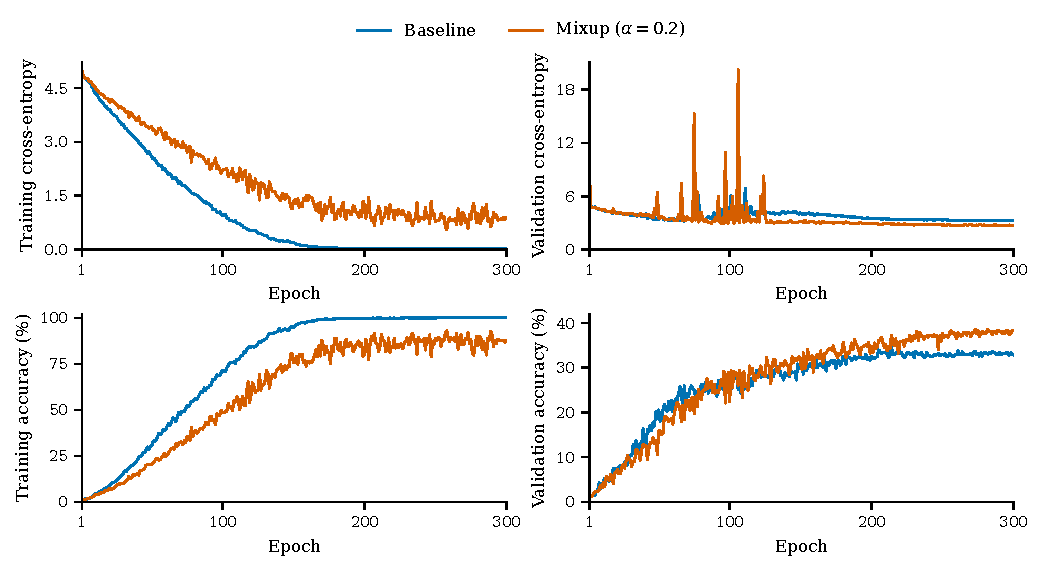
\includegraphics[width=\textwidth]{images/mixup.pdf}
\caption{The selected weight decay baseline and Mixup over 300 epochs. Mixup training loss and accuracy use interpolated targets; validation metrics use the original images and labels.}
\label{fig:mixup}
\end{figure*}

\begin{figure}[ht]
\centering
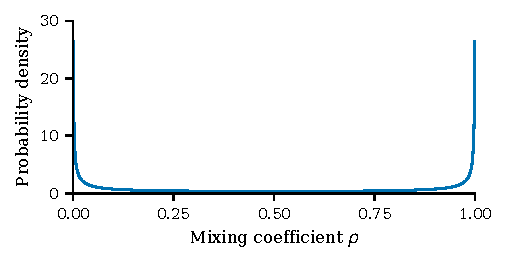
\includegraphics[width=\columnwidth]{images/beta.pdf}
\caption{The $\operatorname{Beta}(0.2,0.2)$ density used for Mixup. The density diverges at both endpoints; the plotted curve is evaluated on $0<\rho<1$.}
\label{fig:beta}
\end{figure}

\section{Mixup and Final Evaluation}

Mixup constructs training examples by interpolating pairs of images and their one-hot labels~\citep{zhang2018mixup}:
\begin{equation}
\begin{aligned}
\widetilde{x}&=\rho x_i+(1-\rho)x_j,\\
\widetilde{y}&=\rho y_i+(1-\rho)y_j,
\end{aligned}
\label{eq:mixup}
\end{equation}
where $\rho\sim\operatorname{Beta}(\alpha,\alpha)$ and $\alpha=0.2$. A random permutation pairs examples within each minibatch, and one coefficient is sampled per minibatch. For logits $z=f(\widetilde{x})$, the training objective is
\begin{equation}
\begin{aligned}
\mathcal{L}_{\mathrm{mix}}={}&\rho\,\mathrm{CE}(z,y_i)\\
&+(1-\rho)\,\mathrm{CE}(z,y_j).
\end{aligned}
\label{eq:mixup-loss}
\end{equation}

The symmetric Beta density is
\begin{equation}
p(\rho)=\frac{\rho^{\alpha-1}(1-\rho)^{\alpha-1}}
{B(\alpha,\alpha)},\qquad 0<\rho<1,
\label{eq:beta}
\end{equation}
where $B$ is the beta function. At $\alpha=0.2$, the exponent $\alpha-1=-0.8$ produces the U-shaped density in Figure~\ref{fig:beta}. Most coefficients lie near zero or one, so the mixed image usually resembles one member of the pair, while coefficients in the interior produce stronger interpolation. The distribution is symmetric and has mean 0.5.

The Mixup run retains the selected cosine schedule, initial learning rate of 0.05, and weight decay of $5\times10^{-4}$, and trains for 300 epochs. Table~\ref{tab:mixup} reports the final metrics. Mixup increases final validation accuracy from 32.88\% to 38.29\% and reduces validation cross-entropy from 3.2910 to 2.7401.

\begin{table}[ht]
\centering
\caption{Final metrics after 300 epochs for the selected baseline and Mixup. Mixup training metrics use the paired-label weights. Accuracy is in percent.}
\label{tab:mixup}
\begin{tabular}{@{}lrrrr@{}}
\toprule
Method & Train CE & Val CE & \shortstack{Train acc.\\(\%)} & \shortstack{Val acc.\\(\%)} \\
\midrule
Baseline & 0.0199 & 3.2910 & 99.99 & 32.88 \\
Mixup & 0.8900 & 2.7401 & 87.66 & 38.29 \\
\bottomrule
\end{tabular}
\end{table}

Figure~\ref{fig:mixup} shows that the Mixup objective maintains higher training loss and lower weighted training accuracy than the unmixed baseline. Interpolated labels assign probability mass to both paired classes, so successful fitting does not require a one-hot prediction for every mixed image. Mixup also constrains predictions between training examples: changes in the image mixture are paired with changes in the target distribution. This encourages smoother behavior between examples and provides a mechanism for the lower validation loss and higher validation accuracy observed in the experiment. Early training is quite uneven, with several spikes in validation loss. The accuracy advantage becomes more consistent in the later epochs.

The best Mixup checkpoint occurs at epoch 273, with validation accuracy of 38.62\% and validation cross-entropy of 2.7151. This exceeds the baseline's best validation accuracy by 3.85 percentage points. The selected checkpoint achieves \textbf{37.55\% test accuracy} and cross-entropy of 2.7505 on the 1,534 test images. The final model therefore uses an initial learning rate of 0.05, cosine annealing, weight decay of $5\times10^{-4}$, and Mixup with $\alpha=0.2$.

\bibliography{references}

\end{document}
